% This file was created by matlab2tikz.
%
%The latest updates can be retrieved from
%  http://www.mathworks.com/matlabcentral/fileexchange/22022-matlab2tikz-matlab2tikz
%where you can also make suggestions and rate matlab2tikz.
%
\definecolor{mycolor1}{rgb}{0.00000,0.44700,0.74100}%
\definecolor{mycolor2}{rgb}{0.85000,0.32500,0.09800}%
\definecolor{mycolor3}{rgb}{0.92900,0.69400,0.12500}%
\definecolor{mycolor4}{rgb}{0.49400,0.18400,0.55600}%
\definecolor{mycolor5}{rgb}{0.46600,0.67400,0.18800}%
%
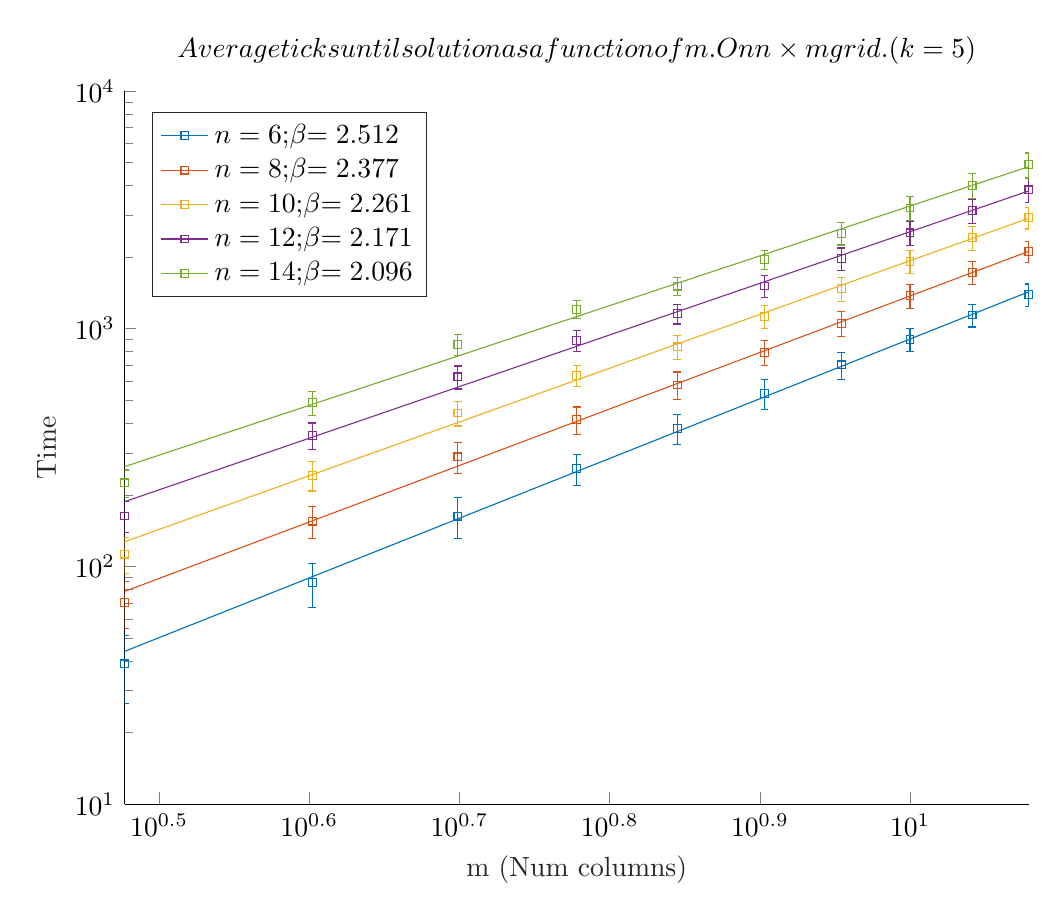
\begin{tikzpicture}

\begin{axis}[%
width=4.521in,
height=3.566in,
at={(0.758in,0.481in)},
scale only axis,
xmode=log,
xmin=3,
xmax=12,
xminorticks=true,
xlabel style={font=\color{white!15!black}},
xlabel={m (Num columns)},
ymode=log,
ymin=10,
ymax=10000,
yminorticks=true,
ylabel style={font=\color{white!15!black}},
ylabel={Time},
axis background/.style={fill=white},
title style={font=\bfseries},
title={$\text{Average ticks until solution as a function of m. On n }\times\text{ m grid. (k = 5)}$},
axis x line*=bottom,
axis y line*=left,
legend style={at={(0.03,0.97)}, anchor=north west, legend cell align=left, align=left, draw=white!15!black}
]
\addplot [color=mycolor1, draw=none, mark size=1.4pt, mark=square, mark options={solid, mycolor1}]
 plot [error bars/.cd, y dir = both, y explicit]
 table[row sep=crcr, y error plus index=2, y error minus index=3]{%
3	38.922	12.3897913565855	12.3897913565855\\
4	85.334	17.8769576614832	17.8769576614832\\
5	162.84	31.3242528663538	31.3242528663538\\
6	257.966	38.9215958723496	38.9215958723496\\
7	379.72	54.2932141819991	54.2932141819991\\
8	533.968	75.359226389368	75.359226389368\\
9	704.074	91.5112733508861	91.5112733508861\\
10	899.646	98.69375663738	98.69375663738\\
11	1141.9	125.53490360871	125.53490360871\\
12	1391.172	150.167329568517	150.167329568517\\
};
\addlegendentry{$\text{n =  6; }\beta\text{ = 2.512}$}

\addplot [color=mycolor1, forget plot]
  table[row sep=crcr]{%
3	43.939038759489\\
4	90.5175507084695\\
5	158.561876123789\\
6	250.683048460023\\
7	369.245036257556\\
8	516.424942178179\\
9	694.252001886417\\
10	904.63459371122\\
11	1149.37987456404\\
12	1430.20859261831\\
};
\addplot [color=mycolor2, draw=none, mark size=1.4pt, mark=square, mark options={solid, mycolor2}]
 plot [error bars/.cd, y dir = both, y explicit]
 table[row sep=crcr, y error plus index=2, y error minus index=3]{%
3	70.482	15.5736557528094	15.5736557528094\\
4	155.078	24.2739028736922	24.2739028736922\\
5	288.784	42.6492586398058	42.6492586398058\\
6	413.962	54.2573153458322	54.2573153458322\\
7	579.478	77.743846878418	77.743846878418\\
8	796.068	94.8381353667378	94.8381353667378\\
9	1054.262	128.311078327802	128.311078327802\\
10	1377.316	161.911082205889	161.911082205889\\
11	1722.83	189.584116884167	189.584116884167\\
12	2111.108	208.158363137993	208.158363137993\\
};
\addlegendentry{$\text{n =  8; }\beta\text{ = 2.377}$}

\addplot [color=mycolor2, forget plot]
  table[row sep=crcr]{%
3	78.4932581498583\\
4	155.510795416505\\
5	264.287082733465\\
6	407.621719226421\\
7	587.979799082659\\
8	807.579902785046\\
9	1068.44972106334\\
10	1372.46379590302\\
11	1721.37047645813\\
12	2116.81193903152\\
};
\addplot [color=mycolor3, draw=none, mark size=1.4pt, mark=square, mark options={solid, mycolor3}]
 plot [error bars/.cd, y dir = both, y explicit]
 table[row sep=crcr, y error plus index=2, y error minus index=3]{%
3	112.686	19.7031935399149	19.7031935399149\\
4	241.676	34.0870485339449	34.0870485339449\\
5	442.154	52.2632296586108	52.2632296586108\\
6	636.586	64.1661998751121	64.1661998751121\\
7	838.246	94.037650136988	94.037650136988\\
8	1126.738	121.729805911677	121.729805911677\\
9	1472.368	175.216363745652	175.216363745652\\
10	1920.808	212.202721769191	212.202721769191\\
11	2413.222	275.802652129822	275.802652129822\\
12	2936.758	310.504417718727	310.504417718727\\
};
\addlegendentry{$\text{n = 10; }\beta\text{ = 2.261}$}

\addplot [color=mycolor3, forget plot]
  table[row sep=crcr]{%
3	127.008518163959\\
4	243.374444751074\\
5	403.045527028873\\
6	608.632010791091\\
7	862.378086764894\\
8	1166.26412011824\\
9	1522.06993194577\\
10	1931.41698763278\\
11	2395.79807588391\\
12	2916.59905898125\\
};
\addplot [color=mycolor4, draw=none, mark size=1.4pt, mark=square, mark options={solid, mycolor4}]
 plot [error bars/.cd, y dir = both, y explicit]
 table[row sep=crcr, y error plus index=2, y error minus index=3]{%
3	162.898	24.1460070262274	24.1460070262274\\
4	355.852	45.1948586289745	45.1948586289745\\
5	627.17	69.6230121989512	69.6230121989512\\
6	893.99	90.6796531698153	90.6796531698153\\
7	1157.482	111.254252473273	111.254252473273\\
8	1512.326	163.924159244353	163.924159244353\\
9	1968.836	216.497851590927	216.497851590927\\
10	2528.112	291.884999892637	291.884999892637\\
11	3138.58	357.788318089233	357.788318089233\\
12	3835.148	441.203684797575	441.203684797575\\
};
\addlegendentry{$\text{n = 12; }\beta\text{ = 2.171}$}

\addplot [color=mycolor4, forget plot]
  table[row sep=crcr]{%
3	187.262730312629\\
4	349.733486127157\\
5	567.757503143877\\
6	843.515698689346\\
7	1178.84893741936\\
8	1575.35717552076\\
9	2034.45984487936\\
10	2557.43556740306\\
11	3145.44976884796\\
12	3799.57470847251\\
};
\addplot [color=mycolor5, draw=none, mark size=1.4pt, mark=square, mark options={solid, mycolor5}]
 plot [error bars/.cd, y dir = both, y explicit]
 table[row sep=crcr, y error plus index=2, y error minus index=3]{%
3	224.602	29.8375628413687	29.8375628413687\\
4	487.724	57.6767981956367	57.6767981956367\\
5	859.618	85.0339557073907	85.0339557073907\\
6	1206.27	103.914452926694	103.914452926694\\
7	1510.346	134.469708443865	134.469708443865\\
8	1952.838	181.569365877756	181.569365877756\\
9	2518.19	269.303856329738	269.303856329738\\
10	3218.688	377.33625847501	377.33625847501\\
11	4006.49	491.819331064587	491.819331064587\\
12	4892.054	588.934300499308	588.934300499308\\
};
\addlegendentry{$\text{n = 14; }\beta\text{ = 2.096}$}

\addplot [color=mycolor5, forget plot]
  table[row sep=crcr]{%
3	262.950218648537\\
4	480.562453077794\\
5	767.14396812945\\
6	1124.2004372353\\
7	1552.98314941824\\
8	2054.56577539883\\
9	2629.89048558783\\
10	3279.79793599745\\
11	4005.04791296568\\
12	4806.33417829283\\
};
\end{axis}
\end{tikzpicture}%